\section*{Appendix: Predicting disability outcomes and utility after treatment of stroke with thrombolysis (IVT) or thrombectomy (MT). Detailed methodology}

\appendix
\setcounter{section}{0}
\renewcommand{\thesection}{A\Alph{section}}
\setcounter{figure}{0}
\renewcommand{\thefigure}{A.\arabic{figure}}
\setcounter{table}{0}
\renewcommand{\thetable}{A.\arabic{table}}

The methodology described here, synthesising data from multiple sources, is for patients with an ischaemic stroke (a stroke that is caused by a clot). These patients can be further defined by the location of the clot: those with a large vessel occlusion (LVO); and those not with a large vessel occlusion (nLVO). Patients with an nLVO can be treated with thrombolysis (IVT), a clot-busting medication. Patients with an LVO can be treated with IVT and/or thrombectomy (MT), which physically removes the clot. The benefit received by the patient from either treatment (IVT and/or MT) are time dependent, such that the sooner they are administered, the better the outcome, with each treatment having no effect after a specified duration (6.3 hours for IVT \cite{emberson_effect_2014}, and 8 hours for MT \cite{fransen_time_2016}). 

This method calculates disability outcome estimates for three patient-treatment cohorts: 

\begin{enumerate}
    \item nLVO-IVT (patients with an nLVO that are treated with IVT).
    \item LVO-IVT (patients with an LVO that are treated with IVT).
    \item LVO-MT (patients with an LVO that are treated with MT
    
\end{enumerate}

The result is provided as a distribution of disability (with seven levels) following reperfusion treatment at any point between these two time stages: 1) receiving reperfusion treatment as soon as their stroke began (this will be referred to as time of stroke onset, and we will use the terminology \textit{t = 0}), and 2) receiving reperfusion treatment at the duration after stroke onset where the treatment has no effect (this will be referred to as time of no effect, and we will use the terminology \textit{t = No Effect}). mRS distributions with treatment include the risk of death associated with treatment.

The method is built by synthesising data from multiple sources (figure \ref{fig:cauldron}), including reperfusion treatment clinical trials \cite{lees_time_2010, emberson_effect_2014, goyal_endovascular_2016, fransen_time_2016, hui_efficacy_2020, de_la_ossa_herrero_design_2013} and 3 years worth of stroke admission data for England and Wales (Sentinel Stroke National Audit Programme, SSNAP) to define the distribution of disability for each of the three patient-treatment cohorts at the two time stages (\textit{t = 0} \& \textit{t = No Effect}), and we use interpolation to determine the disability distribution at any point in-between.

\begin{figure}[h]
    \centering
    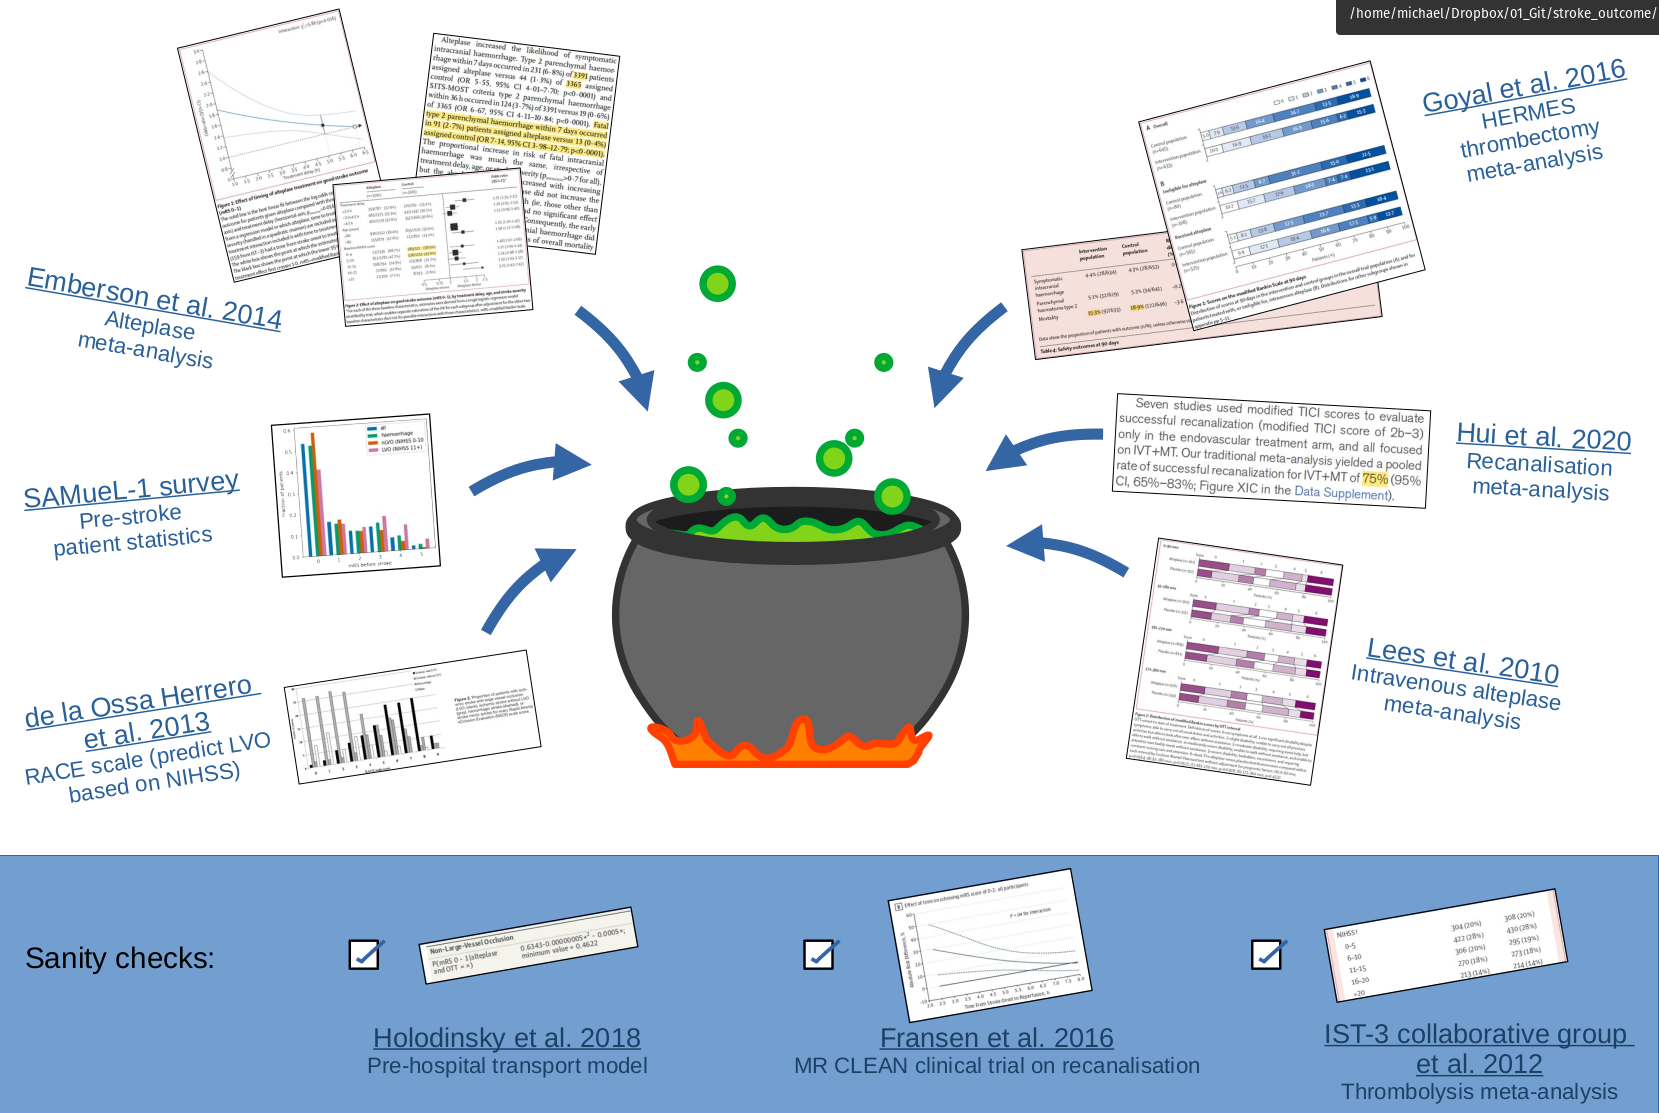
\includegraphics[width=0.95\linewidth]{images/data_cauldron.png}
    \caption{Synthesis of multiple data sources into a disability-level model}
    \label{fig:cauldron}
\end{figure}

\subsection{Modified Rankin Scale}

Modified Rankin Scale (mRS) is the most commonly used instrument to describe post-stroke functional outcome \citeappendix{quinn_functional_2009}. Table \ref{app_tab:mrs} shows a description of the seven level so f mRS along with utilties, from Wang \textit{et al.}\cite{wang_utility-weighted_2020}. Utilities are a measure of the preference or value that an individual or society gives a particular health state, with 1 being full health and 0 being dead (values of less than zero describe states where death is considered preferable).

\begin{minipage}{\textwidth}
\renewcommand*{\arraystretch}{1.5} % adjust row spacing
\begin{longtable}[]{@{}llr@{}}
\caption{A description of modified Rankin Scale score, with Utilities from Wang \textit{et al.}\cite{wang_utility-weighted_2020}}\\
\toprule
mRS & Description. & Utility\tabularnewline
\midrule
\endhead
0 & No symptoms. & 0.97\tabularnewline
1 & No significant disability: Able to carry out all usual activities,
despite some symptoms. & 0.88\tabularnewline
2 & \makecell[l]{Slight disability: Able to look after own affairs without assistance, but unable to carry \\ out all previous activities.} &
0.74\tabularnewline
3 & Moderate disability: Requires some help, but able to walk
unassisted. & 0.55\tabularnewline
4 & \makecell[l]{Moderately severe disability: Unable to attend to own bodily needs without assistance, \\ and unable to walk unassisted.} & 0.20\tabularnewline
5 & Severe disability: Requires constant nursing care and attention,
bedridden, incontinent. & -0.19\tabularnewline
6 & Dead. & 0.00\tabularnewline
\bottomrule
\label{app_tab:mrs}
\end{longtable}
\end{minipage}

\subsection{Excess deaths due to treatment}

\subsubsection{Excess IVT treatment deaths due to fatal intracranial haemorrhage}
\label{excess_deaths_ivt}

We use Emberson's 2.29\% excess deaths from IVT on all patients (nLVO and LVO) \cite{emberson_effect_2014} with the combined nLVO/LVO population from Lees \textit{et al.} \cite{lees_time_2010}. From the available trial data, we assume that the split between nLVO/LVO is the same in both Lees and Emberson (there is a large overlap in trials used by Emberson and Lees):

\begin{itemize}
    \item Lees has 3,670 patients, they provide a granular level of mRS distribution for their population (combined nLVO/LVO) but they do not provide the proportions of the split.
    \item Emberson has 6,756 patients (they have the 3,035 patients from IST-3 in addition to those in Lees, with 51 unaccounted for), they provide the excess deaths by stroke severity. To obtain their value of 2.29\% excess deaths from IVT for all patients, this requires a weighting of 48.27\% nLVO and 51.73\% LVO.
    \item IST-3 has 3,035 patients and provide proportion of patients by stroke severity: 48.24\% nLVO and 51.76\% LVO. This is almost the same that we have calculated in Emberson.
    \item Assuming that Lees contains the other patients in Emberson (those not from IST-3), then it is a fair assumption that Lees has the same split (nLVO/LVO) of patients as Emberson, and so can use 2.29\% excess deaths from IVT for Lees combined nLVO/LVO population.
\end{itemize}

Synthesis of these studies produces results in table \ref{tab:ivt_deaths}

\begin{table}[!ht]
    \caption{Excess deaths due to fatal intracranial haemorrhage in IVT-treated patients}
    \centering
    \begin{tabular}{llll}
    \hline
        NIHSS & Treated & Control & Excess \\ \hline
        0-10 (surrogate for nLVO) & 1.41\% & 0.32\% & 1.10\% \\ 
        11+ (surrogate for LVO) & 3.85\% & 0.45\% & 3.41\% \\
        All & 2.68\% & 0.39\% & 2.29\% \\ \hline
    \end{tabular}
    \label{tab:ivt_deaths}
\end{table}

\subsubsection{Excess MT treatment deaths}
\label{excess_deaths_mt}

Excess deaths in patients treated with MT come from Goyal \textit{et al.} \cite{goyal_endovascular_2016}. The control group in that analysis do not receive MT, but do receive other interventions such as IVT (used in 83\% of patients). No additional IVT-related deaths need to be considered when modelling use of MT as the control group (used to estimate the effect of MT at a time MT is no longer effective) already includes IVT-related excess deaths.

\begin{table}[!ht]
    \caption{Excess deaths in MT-treated patients}
    \centering
    \begin{tabular}{lll}
    \hline
        Treated & Control & Excess \\ \hline
        18.9\% & 15.3\% & 3.6\% \\ \hline
    \end{tabular}
\end{table}


\subsection{Derivation of mRS distributions}

For each stroke type and treatment, we derive mRS distributions for if treatment was given at time of onset (\textit{t = 0}) and if treatment is given at a time no benefit remains (\textit{t = No Effect}). These distributions include the risk of death with treatment (which is considered to be not dependent on time from stroke onset).

\subsubsection{mRS distribution at \textit{t = 0} for nLVO-IVT)}

We assume that the mRS distribution for patients treated at \textit{t = 0} will be a weighted average of a full recovery distribution, and a no-benefit distribution, including a correction for risk of treatment-related death (we assume that risk is independent of the time treatment is given). We need a mRS distribution for each of these, and then take a weighted combination (61\% fully recovered and 39\% no effect), where the weights are derived from data in Emberson \textit{et al.} \cite{emberson_effect_2014} (see paragraph on \textit{weights} below).

The \textbf{mRS distribution for fully recovered nLVO patients with IVT at \textit{t = 0}} is taken as the pre-stroke mRS distribution (this will represent a patient receiving a 100\% effective treatment). This distribution comes from the SSNAP dataset, extracting the patients that have an ischaemic stroke and using NIHSS 0-10 as a surrogate for nLVO. This mRS distribution is then corrected for the excess deaths due to treatment with IVT for nLVO patients (1.10\%, see section \ref{excess_deaths_ivt}).

The \textbf{mRS distribution for nLVO patients for which IVT had no effect} is assumed to be the same as patients that were not treated, but adjusted to include the risk of excess death caused by taking the treatment. Unfortunately there does not exist a large clinical trial for just nLVO patients from which we can take the results for the untreated control group. Instead we use the untreated control group of combined nLVO/LVO data from Lees \textit{et al.} \cite{lees_time_2010}, and from that we remove the contribution of the LVO patients by using the results from the untreated control group of LVO-only data from Goyal \textit{et al.} \cite{goyal_endovascular_2016}. Each mRS distribution (Lees, and Goyal) are adjusted to account for the excess deaths due to IVT treatment; this is 2.29\% for the combined nLVO/LVO patients and 3.41\% for LVO patients (see section \ref{excess_deaths_mt}). Weightings for these two mRS distributions (154\% Lees and -54\% Goyal) are chosen such that once the contribution from the LVO patients have been removed from the combined nLVO/LVO distribution, the remaining mRS distribution matches the P(mRS <= 1, \textit{t = No Effect}) of 0.46 (from the control group in Emberson with NIHSS of 0-10).

The \textbf{weights} used to combine these two mRS distribution (61\% fully recovered and 39\% no effect) were informed by data from Emberson \textit{et al.} \cite{emberson_effect_2014}, and found in order to match the P(mRS 0-1, \textit{t = 0}) of 0.63. It is seen from Emberson that 46\% of patients with NIHSS 0-10 had mRS 0-1 in the untreated group (see figure 2 in Emberson \textit{et al.} \cite{emberson_effect_2014}: (189 + 538)/(321 + 1252)). This translates into a 0.85 odds of a good outcome, which, when multiplied by the odds ratio for mRS 0-1 at \textit{t = 0} (which is 2.0, obtained from extrapolating back to \textit{t = 0} in figure 1 `\textit{Effect of timing of alteplase treatment on good stroke outcome, mRS 0–1}'), gives 1.70, before converting to a probability of 63\%.

\subsubsection{mRS distribution at \textit{t = No Effect} for nLVO-IVT)}

As described above (but repeated here for completeness), the \textbf{mRS distribution for nLVO patients for which IVT had no effect} is assumed to be the same as patients that were not treated, but adjusted to include the risk of excess death caused by taking the treatment. Unfortunately there does not exist a large clinical trial for just nLVO patients from which we can take the results for the untreated control group. Instead we use the untreated control group of combined nLVO/LVO data from Lees \textit{et al.} \cite{lees_time_2010}, and from that we remove the contribution of the LVO patients by using the results from the untreated control group of LVO-only data from Goyal \textit{et al.} \cite{goyal_endovascular_2016}. Each mRS distribution (Lees, and Goyal) are adjusted to account for the excess deaths due to IVT treatment; this is 2.29\% for the combined nLVO/LVO patients and 3.41\% for LVO patients (see section \ref{excess_deaths_mt}). Weightings for these two mRS distributions (154\% Lees and -54\% Goyal) are chosen such that once the contribution from the LVO patients have been removed from the combined nLVO/LVO distribution, the remaining mRS distribution matches the P(mRS 0-1, \textit{t = No Effect}) of 0.46 (from the control group in Emberson with NIHSS of 0-10).

\subsubsection{Plot showing the mRS distribution estimates for \textit{t = 0} and \textit{t = No Effect} (for nLVO-IVT)}

Figure \ref{fig:dist_bars_nLVO_treated_with_IVT} uses a block plot to show the expected mRS distribution for nLVO strokes if IVT is given at either time of stroke onset (\textit{t = 0}, upper plot) or time when the effect of treatment has decayed to zero (\textit{t = No Effect}, lower plot), including excess deaths due to treatment.

\begin{figure}[h]
    \centering
    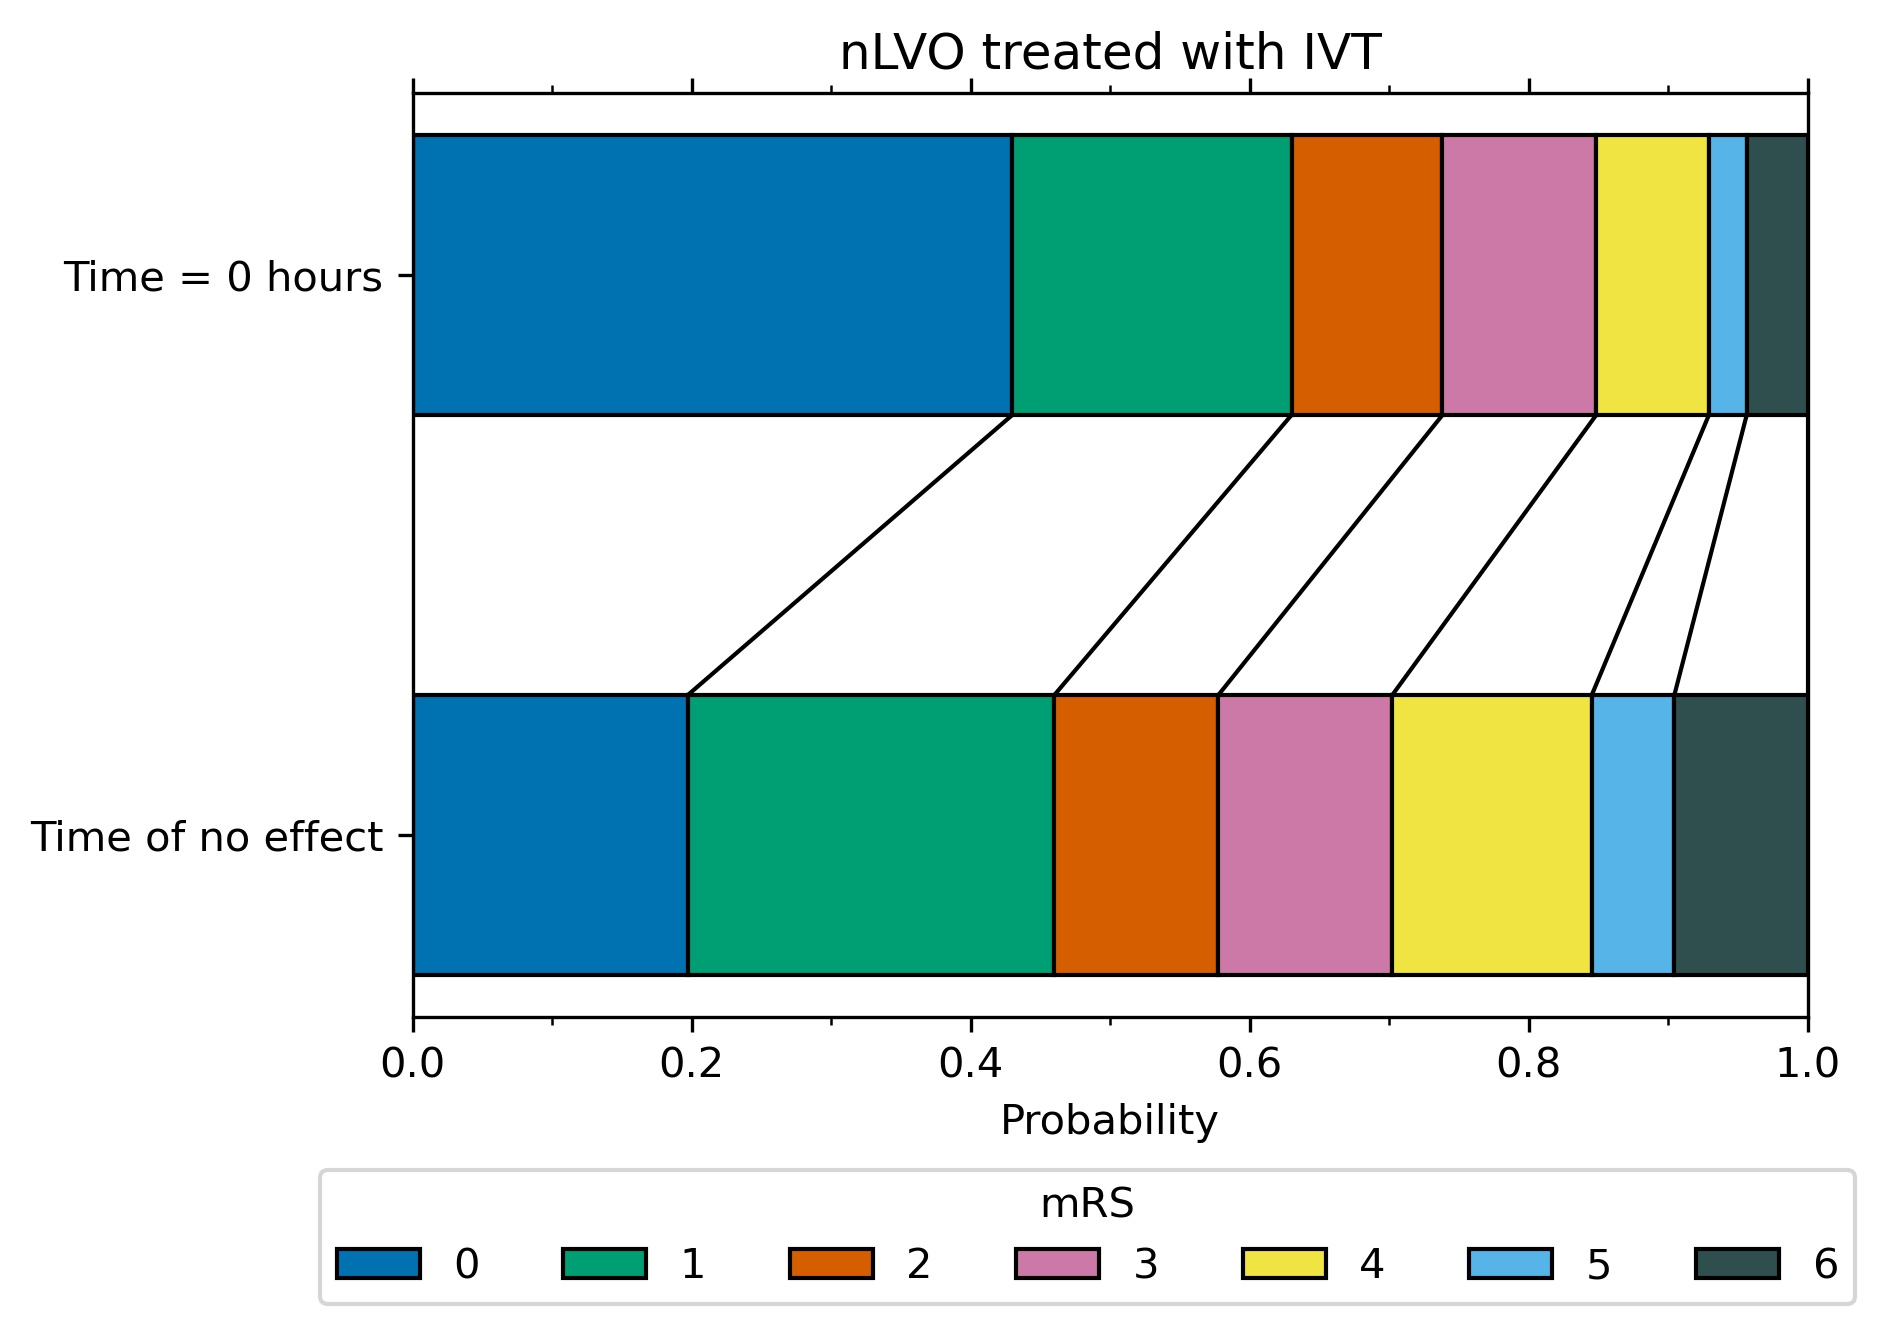
\includegraphics[width=0.75\linewidth]{images/dist_bars_nLVO_treated_with_IVT}
    \caption{Expected mRS distribution for nLVO strokes if IVT given at time of stroke onset (\textit{t = 0}), or if IVT given at time when the effect has decayed to zero (\textit{t = No Effect}). Both distributions include IVT-related excess deaths due to fatal intracranial haemorrhage.}
    \label{fig:dist_bars_nLVO_treated_with_IVT}
\end{figure}

\subsubsection{mRS distribution at \textit{t = 0} for LVO-IVT)}

We assume that the mRS distribution for patients treated at \textit{t = 0} will be a weighted average of a full recovery distribution, and a no-benefit distribution, including a correction for risk of treatment-related death (we assume that risk is independent of the time treatment is given). We need a mRS distribution for each of these, and then take a weighted combination (18\% fully recovered and 82\% no effect), where the weights are derived by data from Emberson \textit{et al.} \cite{emberson_effect_2014} (see paragraph on \textit{weights} below).

The \textbf{mRS distribution for fully recovered LVO patients with IVT at \textit{t = 0}} is taken as the pre-stroke mRS distribution (this will represent a patient receiving a 100\% effective treatment). This distribution comes from the SSNAP dataset, extracting the patients that have an ischaemic stroke and using NIHSS 11+ as a surrogate for LVO. This mRS distribution is then corrected for the excess deaths due to treatment with IVT for LVO patients (3.41\%, see section \ref{excess_deaths_ivt}).

The\textbf{ mRS distribution for LVO patients for which IVT had no effect} is assumed to be the same as patients that were not treated, but adjusted to include the risk of excess death caused by taking the treatment. We obtained this mRS distribution by taking the untreated control group population from Goyal \textit{et al.} \cite{goyal_endovascular_2016}. This distribution is then corrected for the excess deaths due to treatment with IVT for LVO patients (3.41\%, see section \ref{excess_deaths_ivt}).

The \textbf{weights} used to combine these two mRS distributions (18\% fully recovered and 82\% no effect) are chosen to match predicted P(mRS 0-1, \textit{t = 0}) of 0.20, which is set as a target by extrapolating the control group mRS for patients with NIHSS 11+ from Emberson\textit{ et al.} \cite{emberson_effect_2014} back to a predicted odds ratio of mRS 0-1 of 2.0 at \textit{t = 0}.

\subsubsection{mRS distribution at \textit{t = No Effect} for LVO-IVT)}

We assume that patients treated at \textit{t = No Effect} will have the same mRS distribution as patients that were not treated, with an adjustment to include the risk of excess deaths caused by taking the treatment. We obtained this mRS distribution by taking the untreated control population from Goyal \textit{et al.} \cite{goyal_endovascular_2016}. This distribution is then corrected for the excess deaths due to treatment with IVT for LVO patients (3.41\%, see section \ref{excess_deaths_ivt).

\subsubsection{Plot showing the mRS distribution estimates for \textit{t = 0} and \textit{t = No Effect} (for LVO-IVT)}

Figure \ref{fig:dist_bars_nLVO_treated_with_IVT} uses a block plot to show the expected mRS distribution for LVO strokes if IVT is given at either time of stroke onset (\textit{t = 0}, upper plot) or time when the effect of treatment has decayed to zero (\textit{t = No Effect}, lower plot), including excess deaths due to treatment.

\begin{figure}[h]
    \centering
    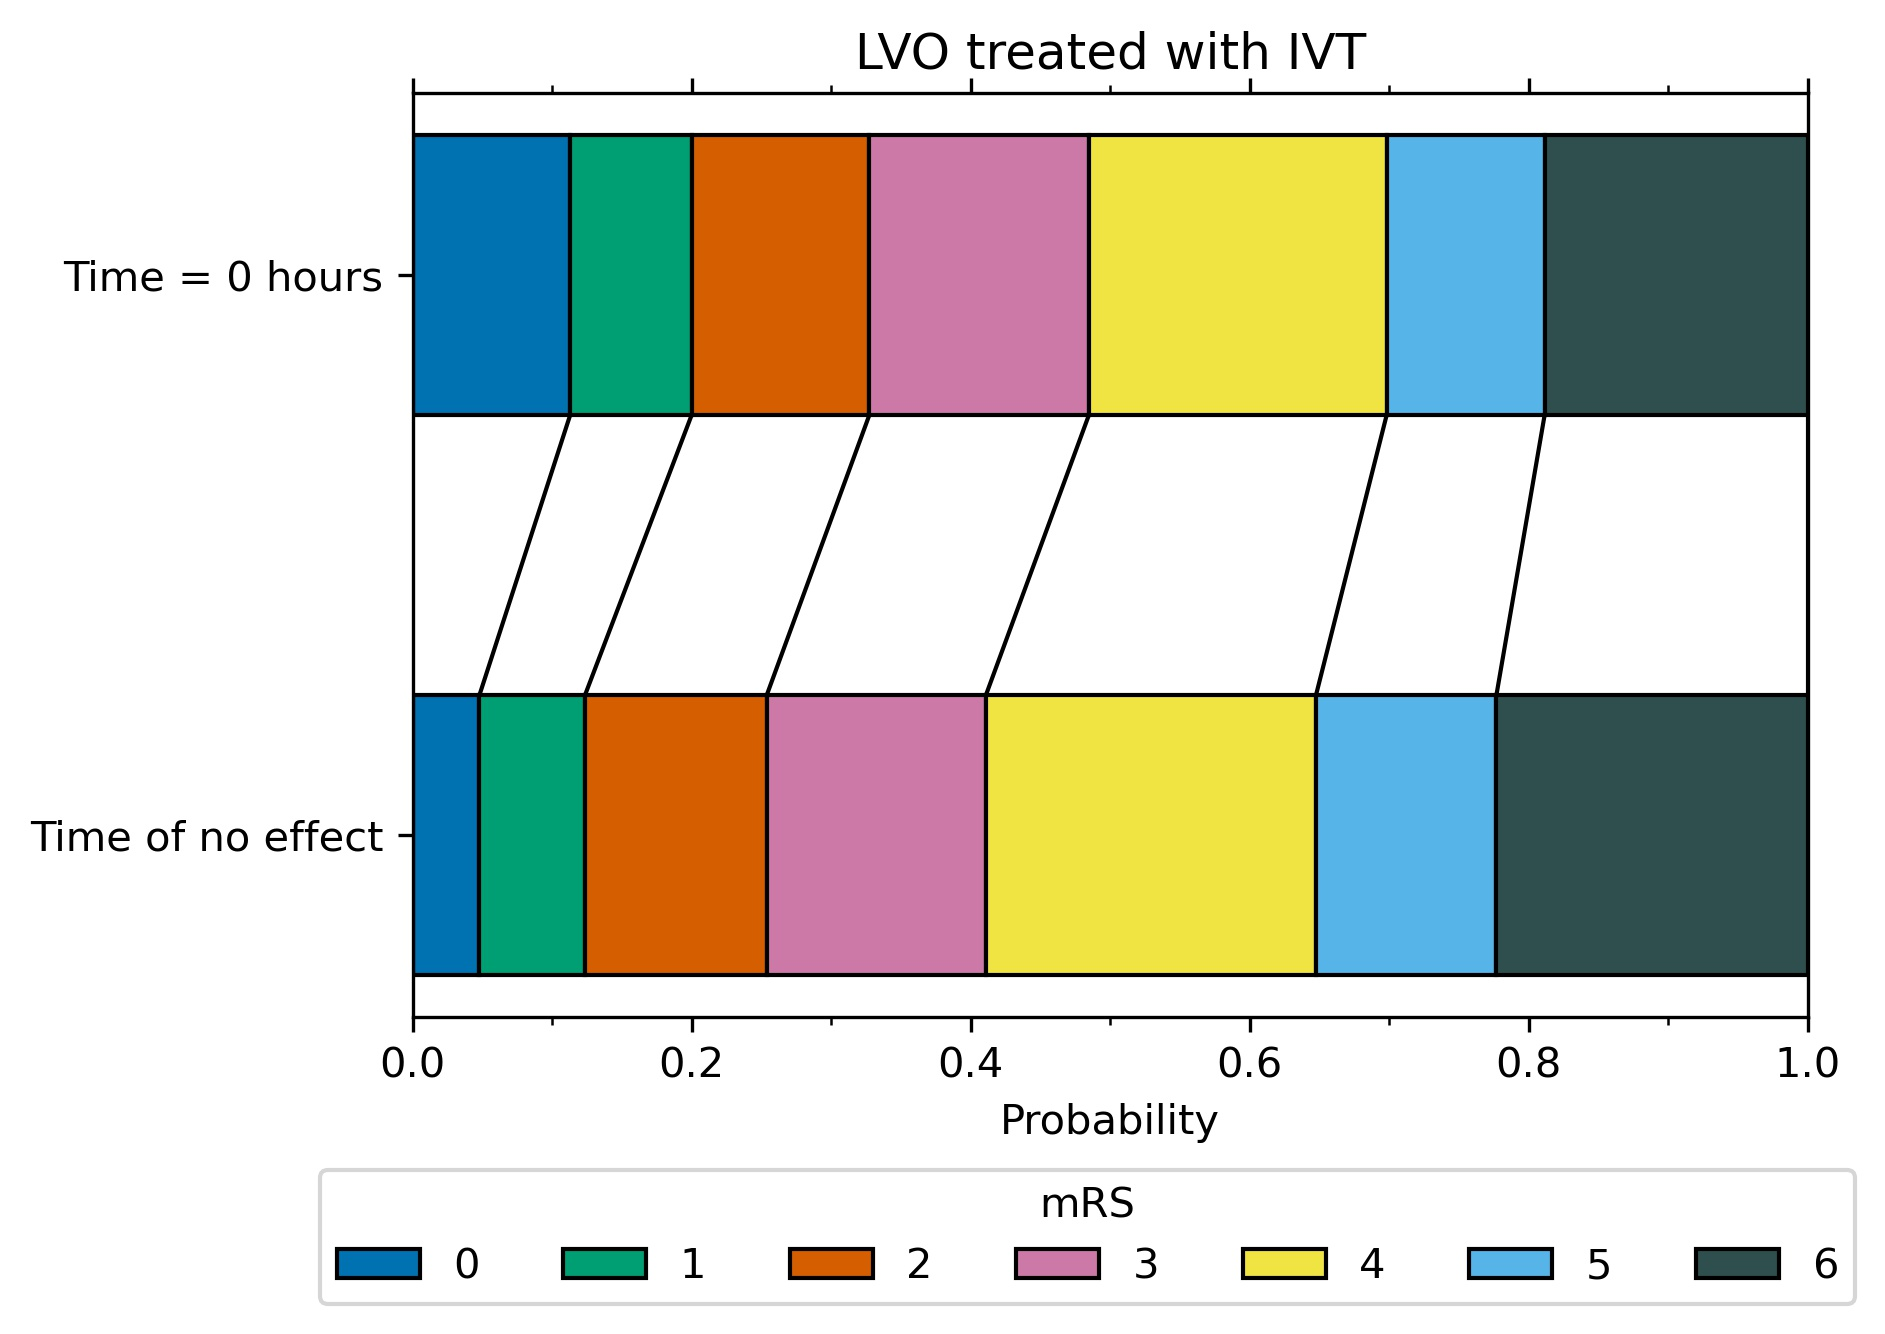
\includegraphics[width=0.75\linewidth]{images/dist_bars_LVO_treated_with_IVT}
    \caption{Expected mRS distribution for LVO strokes if IVT given at time of stroke onset (\textit{t = 0}), or if IVT given at time when the effect has decayed to zero (\textit{t = No Effect}). Both distributions include IVT-related excess deaths due to fatal intracranial haemorrhage.}
    \label{fig:dist_bars_LVO_treated_with_IVT}
\end{figure}

\subsubsection{mRS distribution at \textit{t = 0} for LVO-MT)}

We assume that the mRS distribution for patients treated at \textit{t = 0} will be a weighted average of a full recovery distribution, and a no-benefit distribution, including a correction for risk of treatment-related death (we assume that risk is independent of the time treatment is given). We need a mRS distribution for each of these, and then take a weighted combination (75\% fully recovered and 25\% no effect), where the weights are taken from Hui\textit{ et al.} \cite{hui_efficacy_2020}.

The \textbf{mRS distribution for fully recovered LVO patients with MT at \textit{t = 0}} is taken as the pre-stroke mRS distribution (this will represent a patient receiving a 100\% effective treatment). This distribution comes from the SSNAP dataset, extracting the patients that have an ischaemic stroke and using NIHSS 11+ as a surrogate for LVO. This distribution is then corrected for the excess deaths due to treatment with MT (3.6\%, see section \ref{excess_deaths_mt}).

The \textbf{mRS distribution for LVO patients for which MT had no effect} is assumed to be the same as patients that were not treated, but adjusted to include the risk of excess death caused by taking the treatment. We obtained this mRS distribution by taking the untreated control population from Goyal \textit{et al.} 2016. This distribution is then corrected for the deaths due to treatment with MT (3.6\, see section \ref{excess_deaths_mt}).

The \textbf{weights} used to combine these two mRS distributions (75\% fully recovered and 25\% no effect) are taken from Hui \textit{et al.} \cite{hui_efficacy_2020}, who reported 75\% successful recanalisation with thrombectomy*.

*Extrapolating results of good outcome, when recanalisation has been achieved with MT, from Fransen \textit{et al}. \cite{fransen_time_2016} back to\textit{ t = 0}, assuming 75\% recanalisation, gives the same proportion of patients with mRS 0-2 as the pre-stroke mRS in the SSNAP data (therefore this extrapolation would suggest full recovery of all health with MT theoretically carried out at \textit{t = 0}).

\subsubsection{mRS distribution at \textit{t = No Effect} for LVO-MT)}

We assume that patients treated at *t = No Effect* will have the same mRS distribution as patients that were not treated, and adjusted to include the risk of excess deaths caused by taking the treatment. We obtained this mRS distribution by taking the untreated control population from Goyal et al. 2016. This distribution is then corrected for the excess deaths due to treatment with MT (3.6\%, see section \ref{excess_deaths_ivt).

\subsubsection{Plot showing the mRS distribution estimates for \textit{t = 0} and \textit{t = No Effect} (for LVO-MT)}

Figure \ref{fig:dist_bars_LVO_treated_with_MT} uses a block plot to show the expected mRS distribution for LVO strokes if MT is given at either time of stroke onset (\textit{t = 0}, upper plot) or time when the effect of treatment has decayed to zero (\textit{t = No Effect}, lower plot), including excess deaths due to treatment.

\begin{figure}[h]
    \centering
    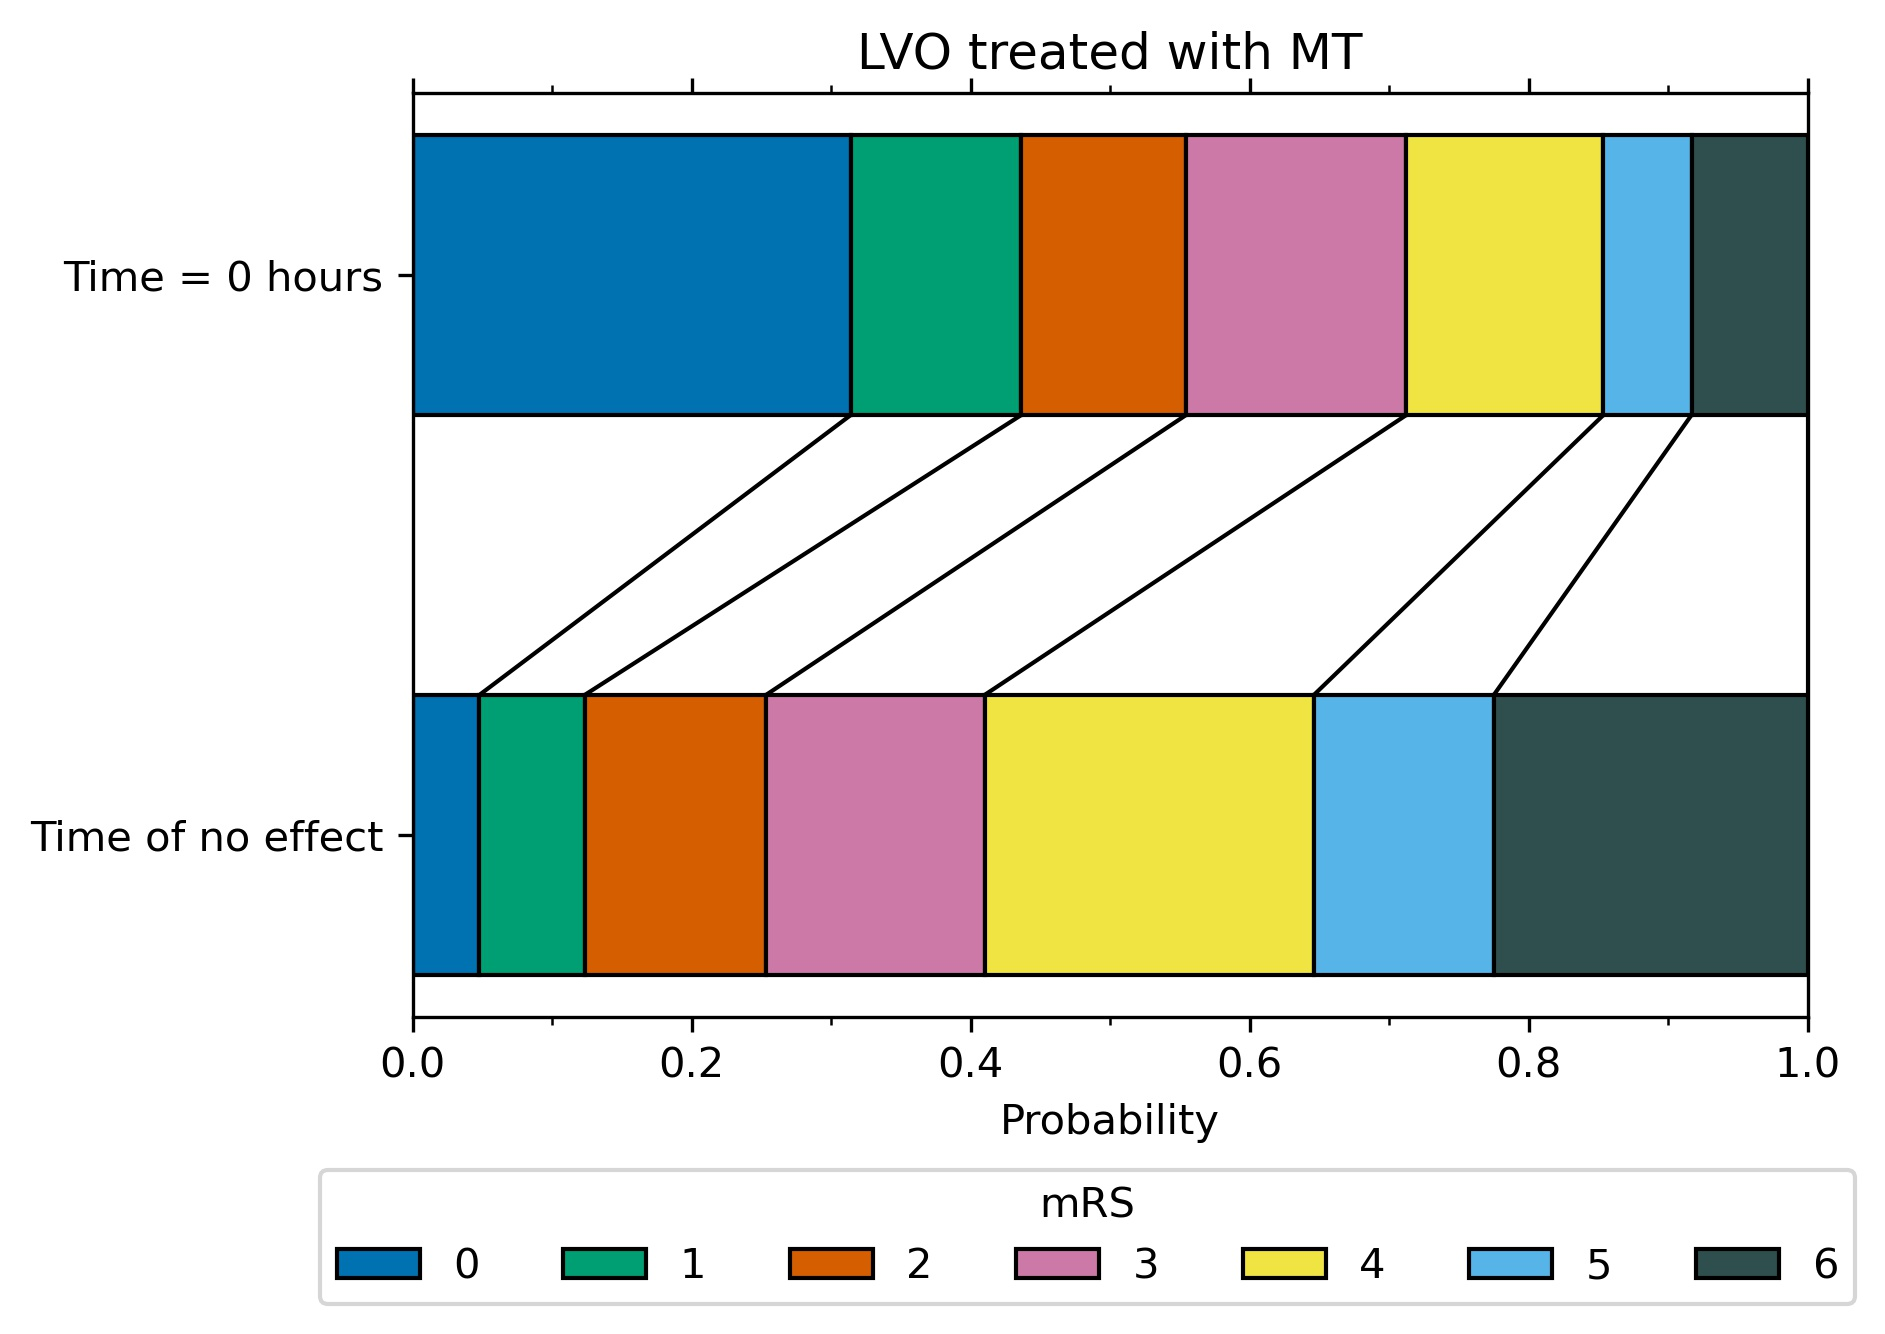
\includegraphics[width=0.75\linewidth]{images/dist_bars_LVO_treated_with_MT}
    \caption{Expected mRS distribution for LVO strokes if MT given at time of stroke onset (\textit{t = 0}), or if MT given at time when the effect has decayed to zero (\textit{t = No Effect}). Both distributions include MT-related excess deaths due to fatal intracranial haemorrhage.}
    \label{fig:dist_bars_LVO_treated_with_IVT}
\end{figure}

\subsection{Interpolation of distributions depending on time to treatment}

% mRS distribution derivation

We define outcome in terms of probability distributions of mRS scores. 

We use these outcome probability distributions to model the variation of outcome probability with time for each combination of occlusion type and treatment.
% 
For a given mRS category $x$ at time $t$, the probability values, $P(\mRS\leq x\ |\ t)$, can be converted to odds, $O(\mRS\leq x\ |\ t)$, and \logodds, $\log_e[O(\mRS\leq x\ |\ t)]$, by using the standard definition $O=P/(1-P)$.
The \logodds\ can be modelled similarly to outcome \logoddsratio, which falls off approximately linearly with time\cite{emberson_effect_2014, fransen_time_2016}. 
% 
The known relation between \logodds\ and time can then be converted back into relations for odds and probability with time.

% Maths description:
We define a straight line fit $\log_e[O(\mRS\leq x\ |\ t)] = A_x + b_x t$
for constants $A_x$ and $b_x$ that differ for each mRS category $x$, $0\leq x \leq5$.
This gives an exponential form of odds where $O(\mRS\leq x\ |\ t) = \exp{(A_x + b_x t)}$.
The conversion to probability uses the inversion of the standard relation between probability and odds,  $P=O/(1+P)$. 
The final result is probability in the form of a logistic function:

\begin{equation}
P(\mRS\leq x\ |\ t) = \frac{1}{1+\exp{(A_x + b_x t)}}
\end{equation}


The constants $A_x$ and $b_x$ are found by considering the known data at $t=0$ and $t=\tne$. 
When $t=0$ then $A_x = \log_e[O(\mRS\leq x\ |\ t=0)]$ and when $t=\tne$ then $b_x = (\log_e[O(\mRS\leq x\ |\ t=\tne)] - A_x) / \tne$. 

\subsubsection{Decay of effect of IVT in nLVO}

Figure \ref{fig:probs_with_time_nLVO_treated_with_IVT} shows the calculated decay of the effect of IVT in patients with nLVO stroke.

\begin{figure}[h!]
    \centering
    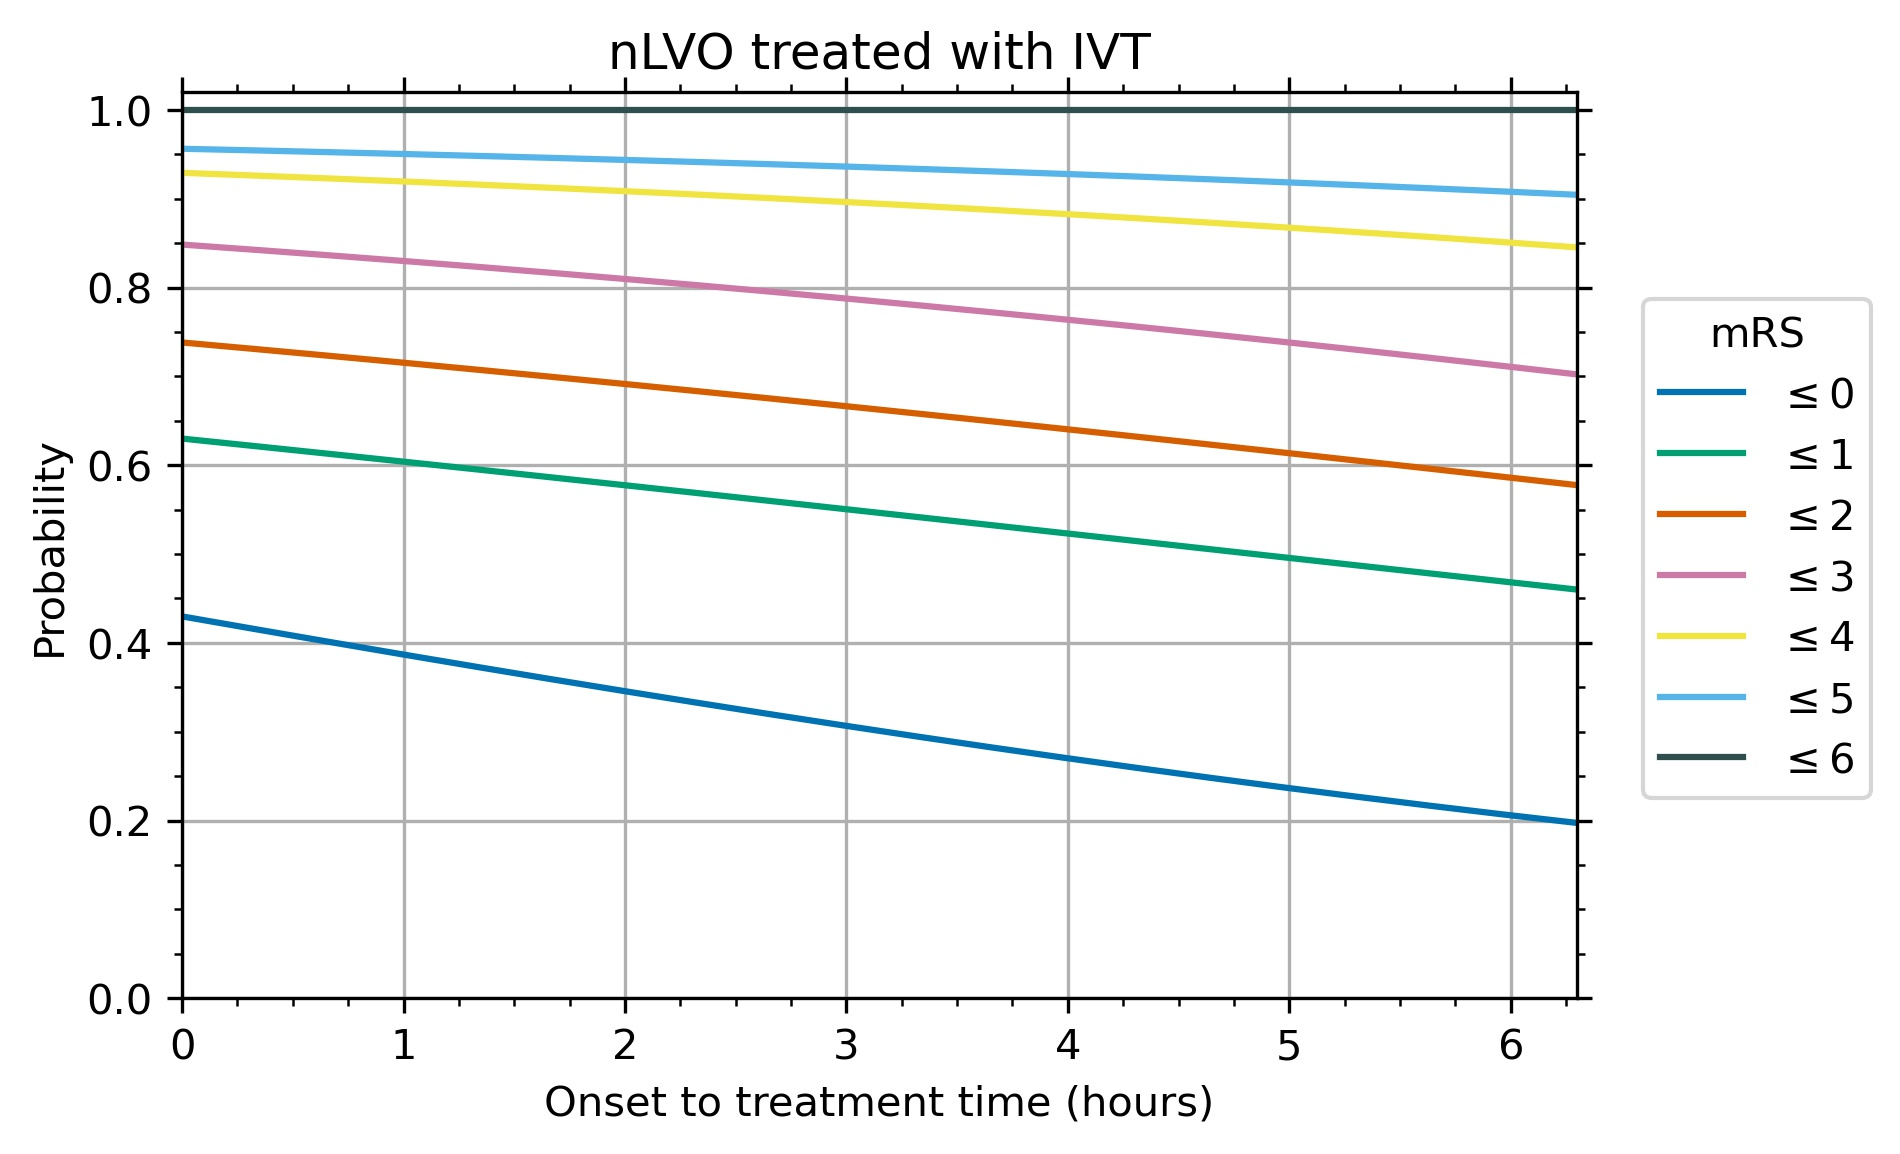
\includegraphics[width=0.65\linewidth]{images/probs_with_time_nLVO_treated_with_IVT}
    \caption{Modelled mRS distribution for nLVO strokes depending on time to treatment with IVT.}
    \label{fig:probs_with_time_nLVO_treated_with_IVT}
\end{figure}

\subsubsection{Decay of effect of IVT in LVO}

Figure \ref{fig:probs_with_time_LVO_treated_with_IVT} shows the calculated decay of the effect of IVT in patients with LVO stroke.

\begin{figure}[h!]
    \centering
    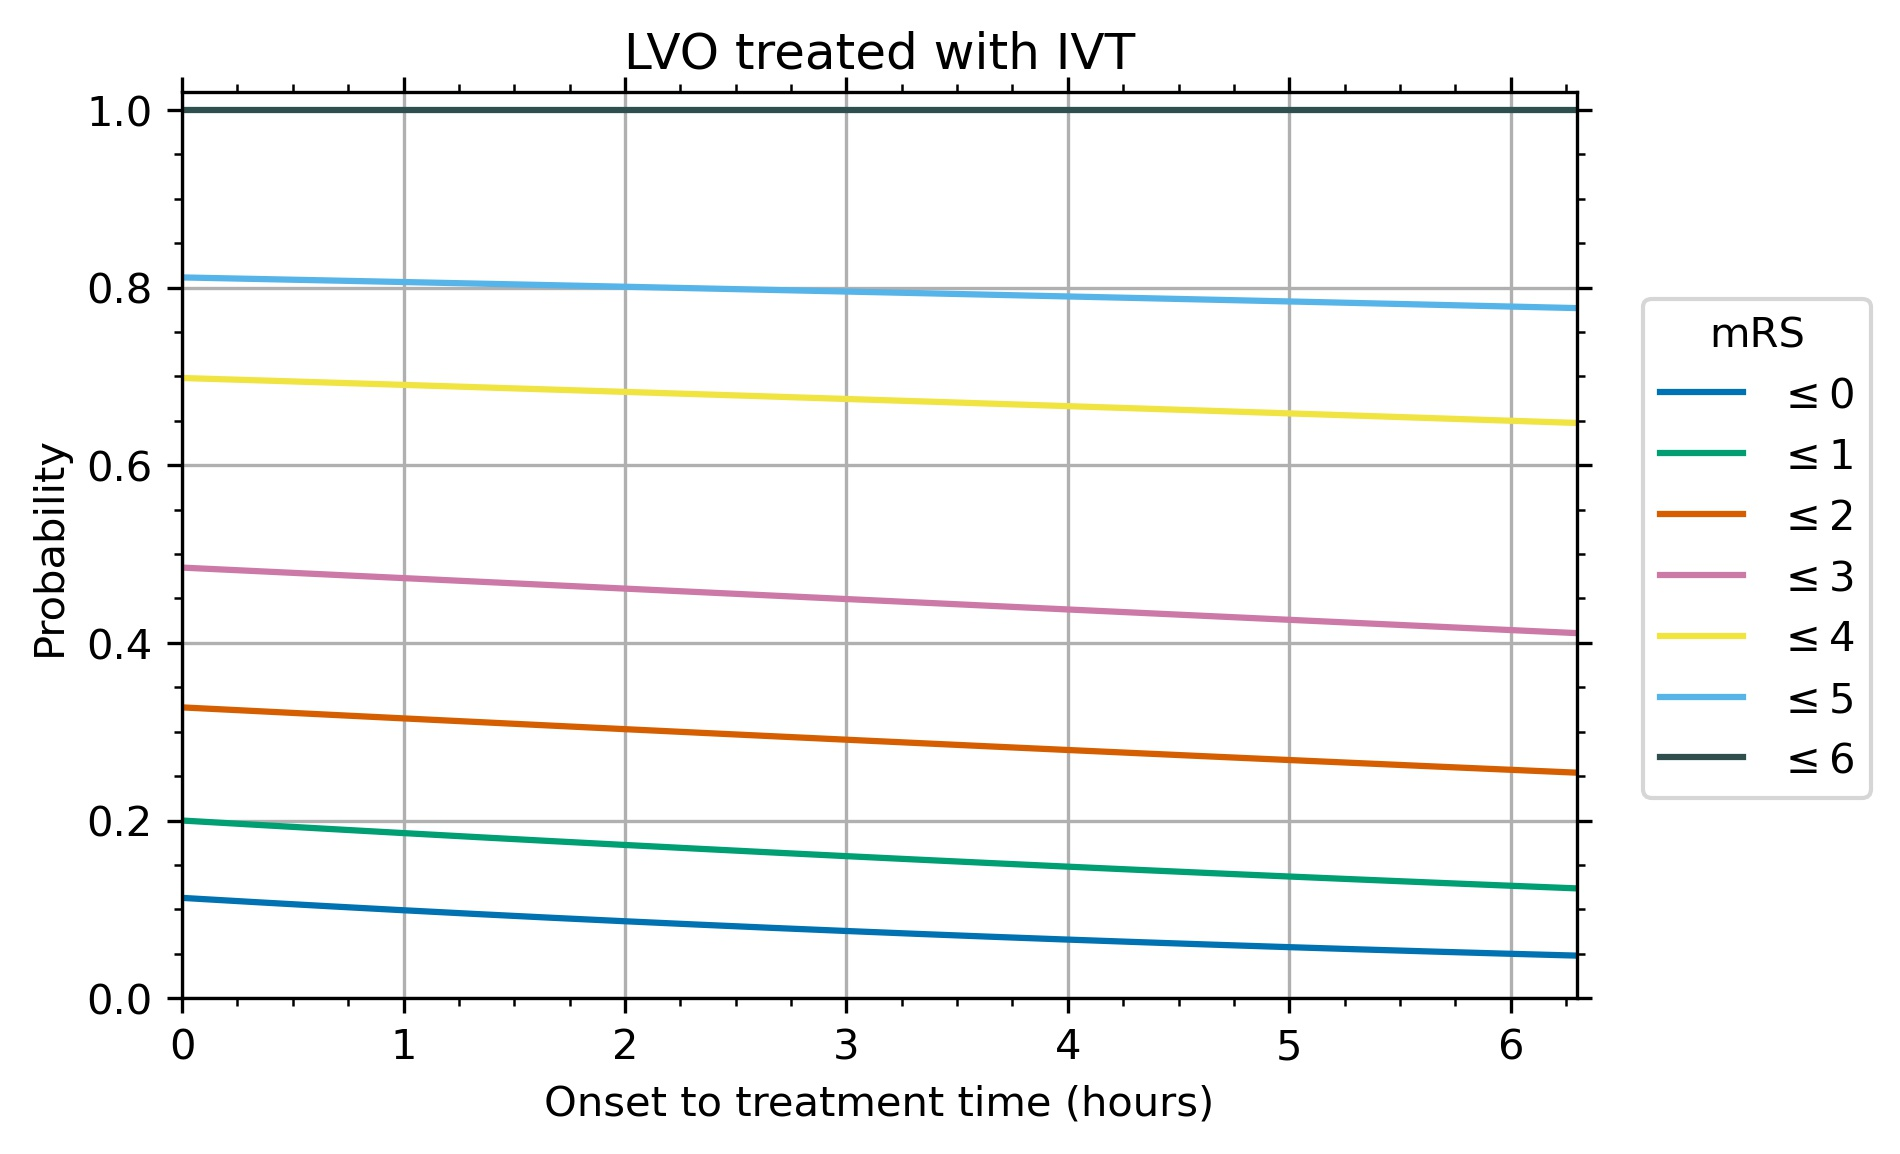
\includegraphics[width=0.65\linewidth]{images/probs_with_time_LVO_treated_with_IVT}
    \caption{Modelled mRS distribution for LVO strokes depending on time to treatment with IVT.}
    \label{fig:probs_with_time_LVO_treated_with_IVT}
\end{figure}

Figure \ref{fig:probs_with_time_LVO_treated_with_IVT} shows the calculated decay of the effect of MT in patients with LVO stroke.

\begin{figure}[h!]
    \centering
    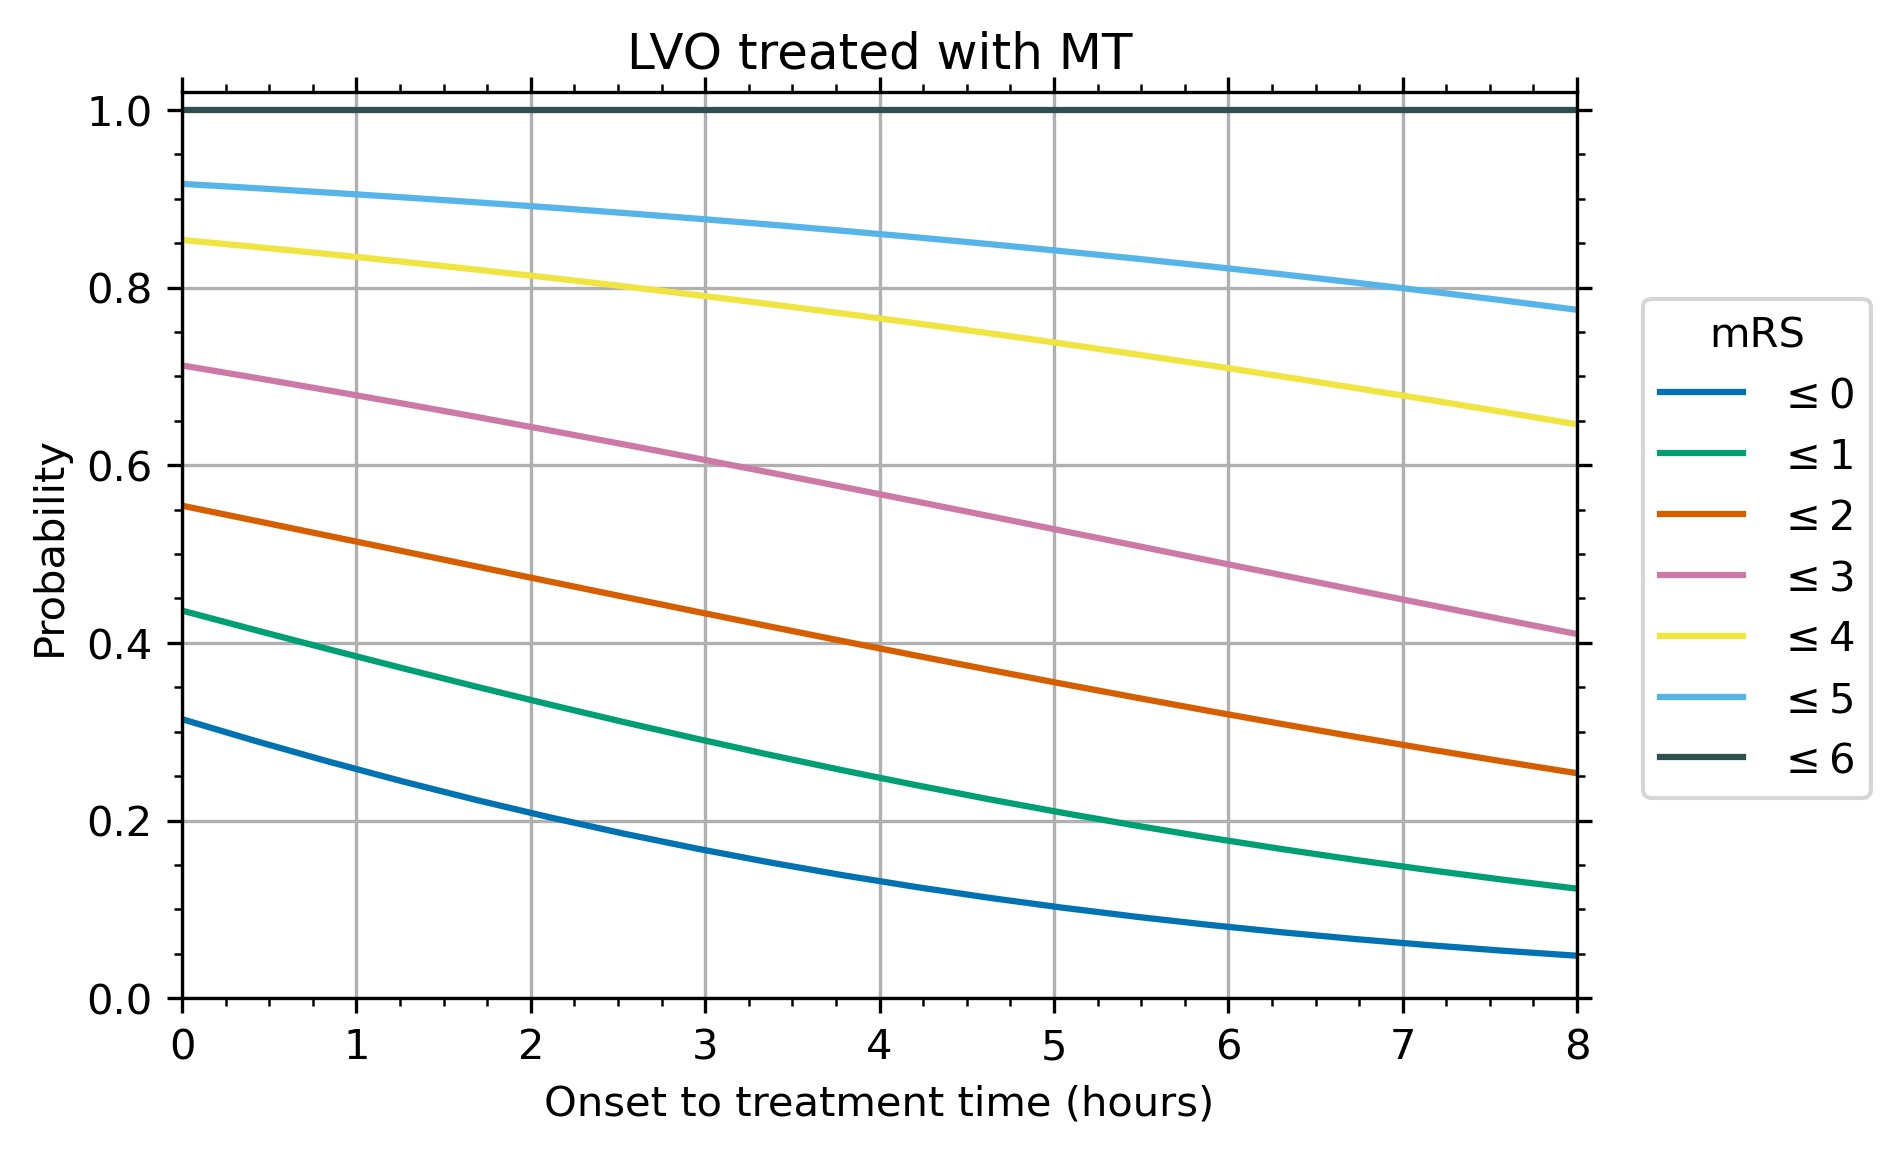
\includegraphics[width=0.65\linewidth]{images/probs_with_time_LVO_treated_with_MT}
    \caption{Modelled mRS distribution for LVO strokes depending on time to treatment with MT.}
    \label{fig:probs_with_time_LVO_treated_with_MT}
\end{figure}

\subsection{Summary plots}

The effect of time to treatment with IVT or MT, in isolation is shown in figure \ref{fig:time_to_treatment}. The combined effect of IVT and MT in a mixed nLVO/LVO population is shown in figure \ref{fig:matrix_utility_and_mRS}

\begin{figure}[h!]
    \centering
    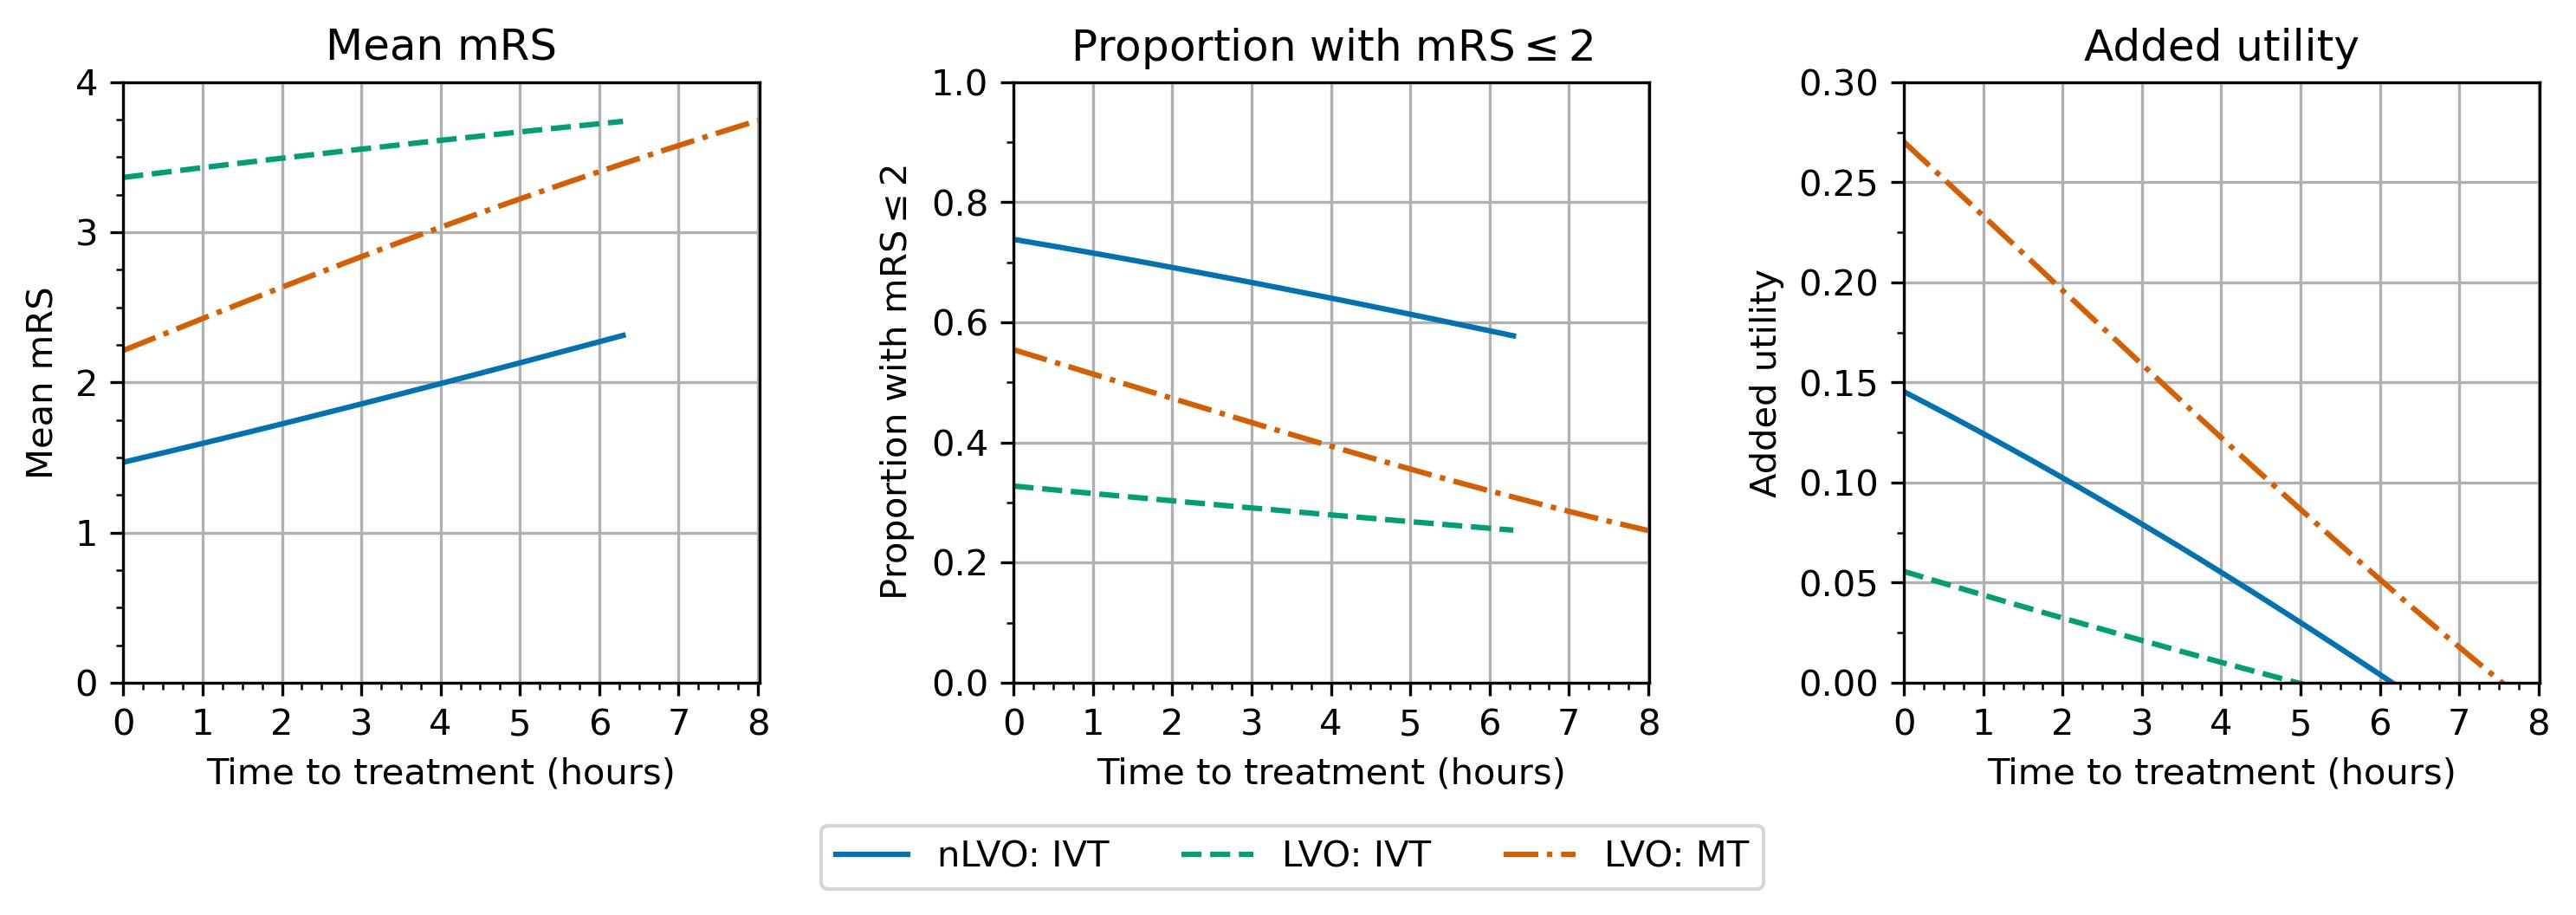
\includegraphics[width=1.0\linewidth]{images/time_to_treatment}
    \caption{The effect of time to treatment on effectiveness of treatment, shown individually for nLVO treated with IVT, and LVO treated with MT or IVT alone (the effect of MT is based on clinical trails where 85\% of patients had previously received IVT). Effectiveness is shown as mean mRS (left) , the proportion of patients with mRS 0-2 (middle), and added utility (right).}
    \label{fig:time_to_treatment}
\end{figure}


\begin{figure}[h!]
    \centering
    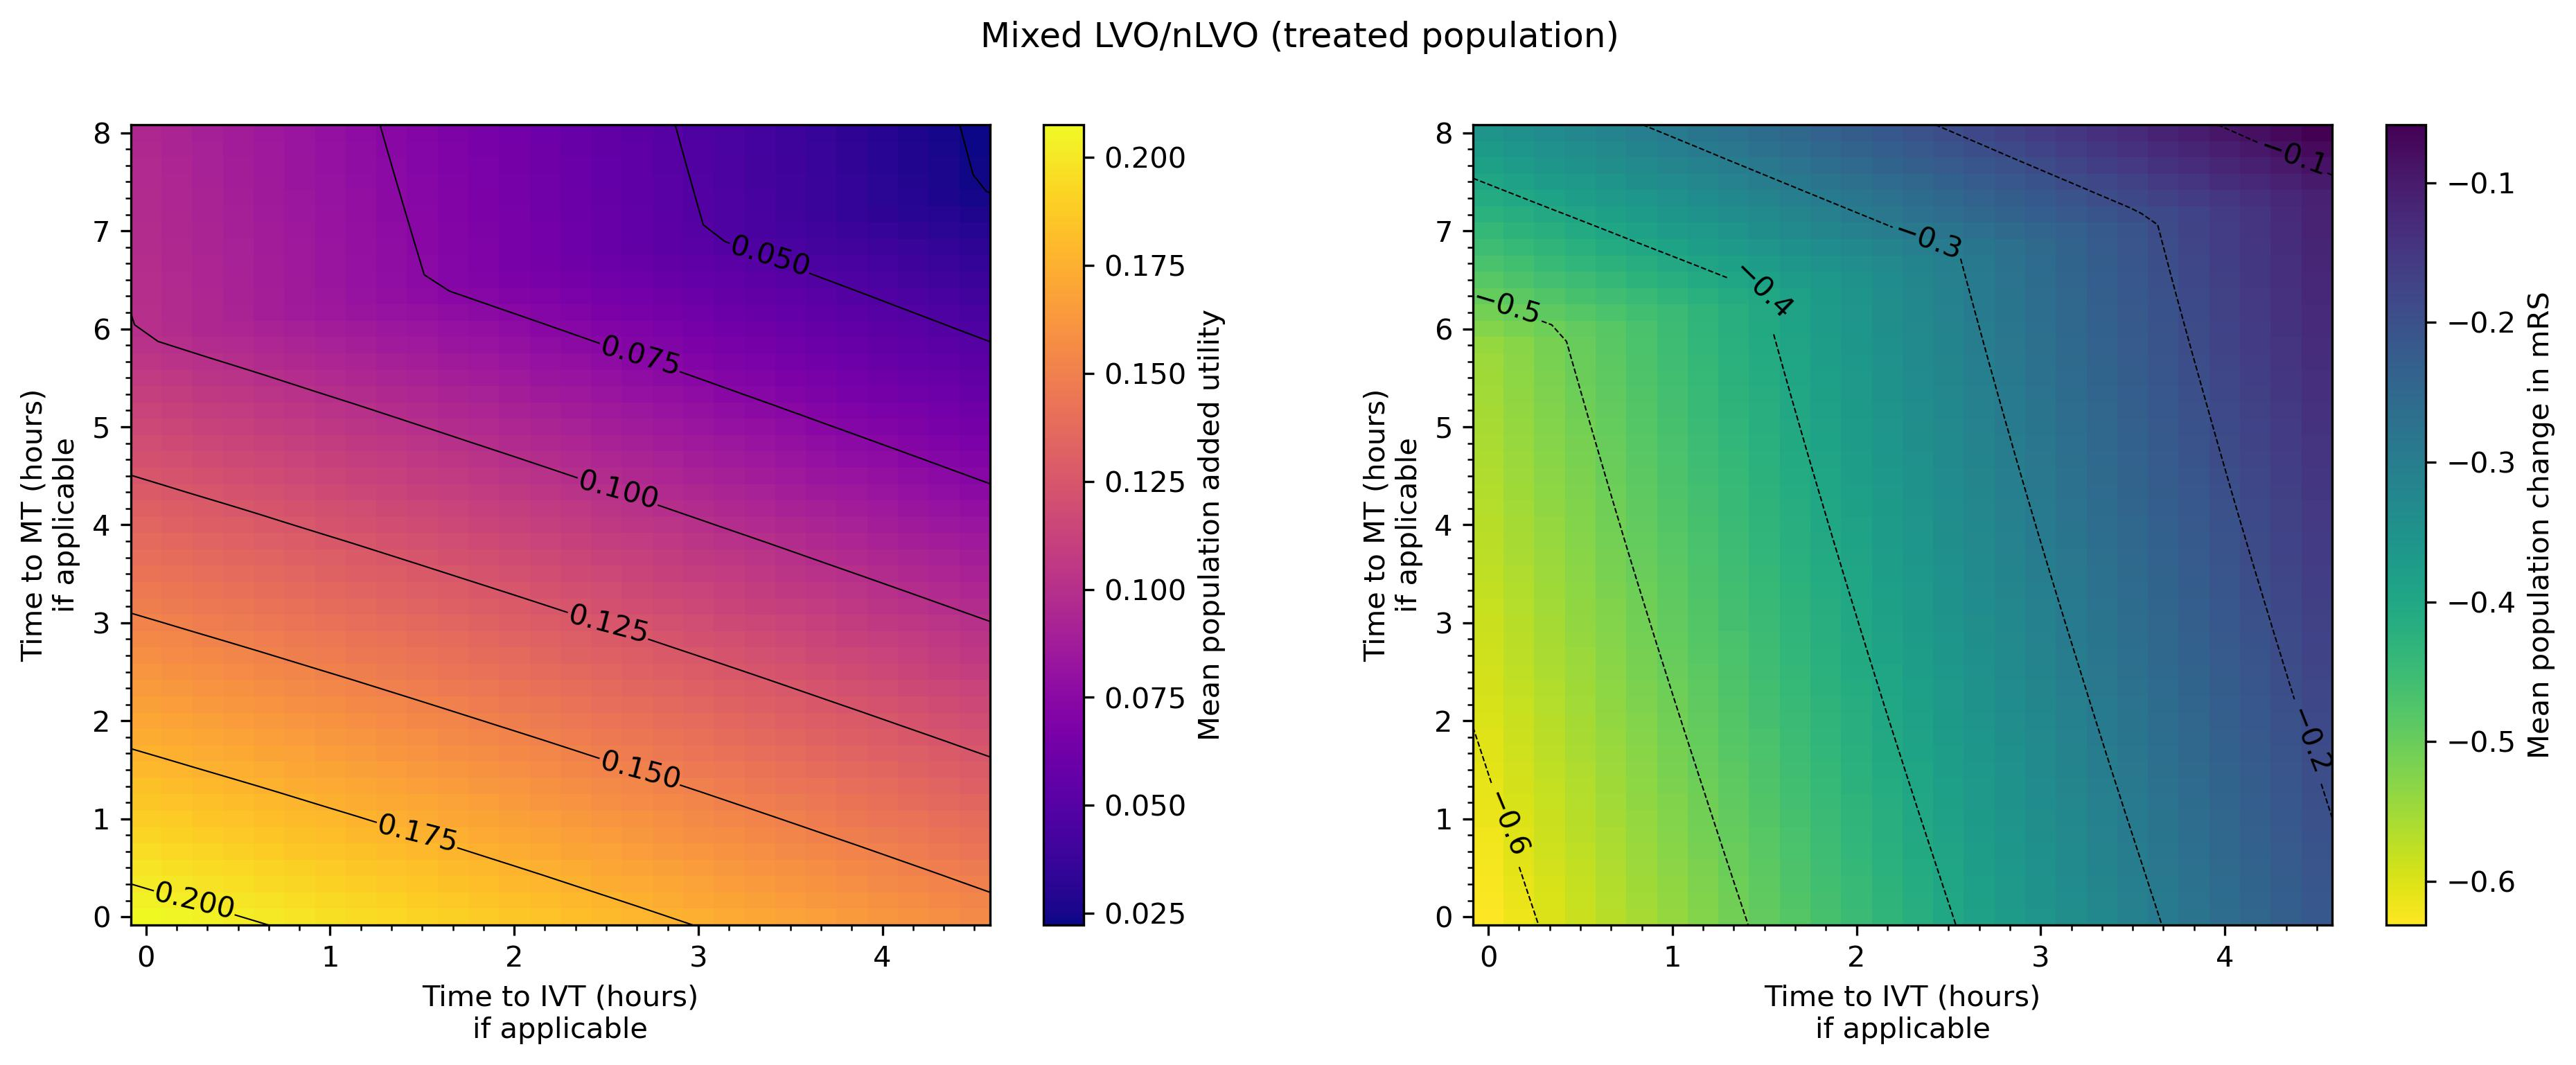
\includegraphics[width=1.0\linewidth]{images/matrix_utility_and_mRS}
    \caption{The effect of time to treatment on effectiveness of treatment, shown individually for nLVO treated with IVT, and LVO treated with MT or IVT alone (the effect of MT is based on clinical trails where 85\% of patients had previously received IVT). Effectiveness is shown as mean mRS (left) , the proportion of patients with mRS 0-2 (middle), and added utility (The effect of time to treatment with IVT and MT on a mixed nLVO/LVO population (LVO making up 35\% of all treated ischaemic strokes).}
    \label{fig:matrix_utility_and_mRS}
\end{figure}

\subsection{Packaging of the method for Python}

The method described here is available as a Python package at: \url{https://pypi.org/project/stroke-outcome/}. This method will also apply Utility weighting (defaulting to the Utilities described by Wang \textit{et al.} \cite{wang_utility-weighted_2020}.

Further description of the method is available at \url{https://samuel-book.github.io/stroke_outcome/}


\bibliographystyle{naturemag}
\bibliography{refs}